% ai-phishing-detection-dissertation/report/sections/4-results/xai-for-distilbert-using-lime.tex

\subsection{XAI for DistilBERT using LIME}
The following examples below demonstrate the LIME out, highlighting keywords that steered the final decision of the DistilBERT model to the "Phishing" (label 1) class.\newline

\noindent Instance 0: Phishing email with persuasive language

\begin{itemize}
  \item \textbf{Original text snippet}: "\textit{do you have a crying need for bigger and stronger love weapon? we'll tell where to get it! see your tool swell in length and width immensely! the herbert henry dow high school located in midland,he cheered on for alberta's kevin martin. martin won 9 8champions league earlier today after defeating li:won}"
  \item \textbf{Model prediction}: Phishing (predicted class index: 1)
\end{itemize}

\noindent The below figure presents the LIME explanation for Instance 1 for sample email classified as phishing. Here, LIME highlighted terms like "\textit{love}" (approx. weight \textbf{0.056}), "\textit{length}" (approx. weight \textbf{0.051}), "\textit{width}" (approx. weight \textbf{0.037}), "\textit{crying}" (approx. weight \textbf{0.033}), "\textit{stronger}" (approx. weight \textbf{0.033}), and "\textit{bigger}" (approx. weight \textbf{0.028}) as the major influential factors to the classification. It suggests these words are common for deceptive content and aim to invoke an emotional response.

\newpage

\vspace{0.5cm}
\begin{figure}[H]
  \begin{center}
    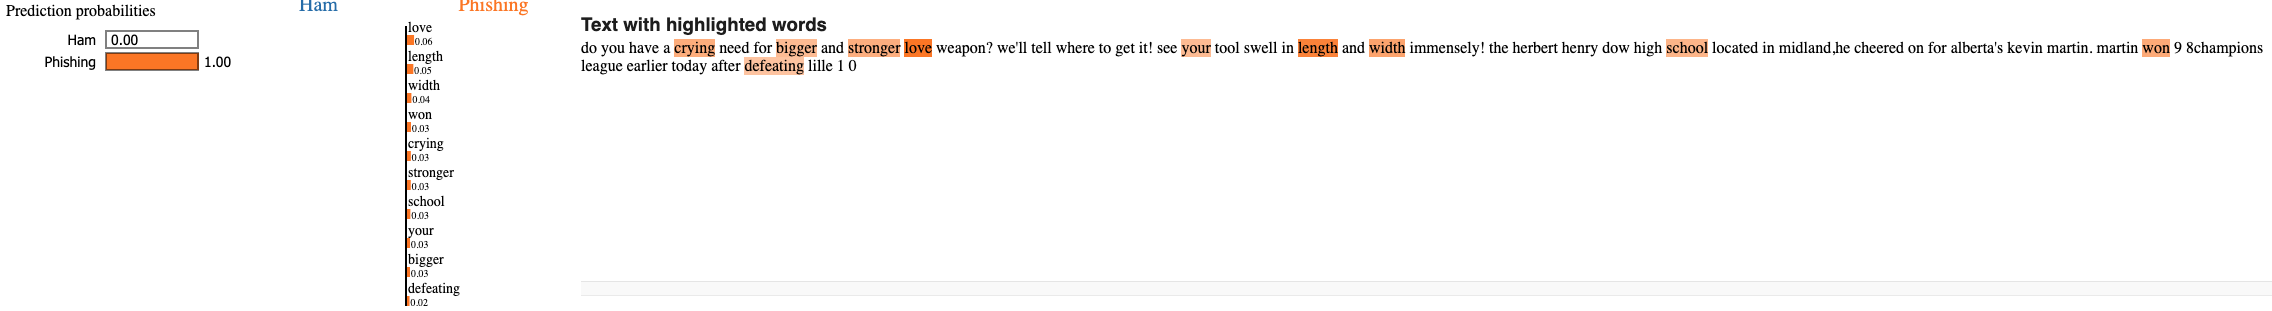
\includegraphics[scale=0.3,angle=90]{xai-visualisations/distilbert/Screenshot 2025-05-26 at 16.11.57.png}
    \caption{DistilBERT LIME explanation for Instance 0}
  \end{center}
\end{figure}

\newpage

\noindent Instance 1: Phishing with potentially misleading content

\begin{itemize}
  \item \textbf{Original text snippet}: "\textit{the daily top 10 from cnn.com top videos and stories as of aug 1, 2008 3 58 pm edt top 10 videos 1. mom parties at a club nancy grace has new photos of casey anthony partying at a nightclub after her daughter caylee vanished. 2. woman's computer spies on her 3. tigers attack teen at zoo 4. mistress}"
  \item \textbf{Model prediction}: Phishing (predicted class index: 1)
\end{itemize}

\noindent Another email that the DistilBERT model classified as phishing, due to terms LIME identified: "\textit{cnn}" (approx. weight \textbf{0.087}), "\textit{videos}" (approx. weight \textbf{0.065}), "\textit{starbucks}" (approx. weight \textbf{0.051}), "\textit{2008}" (approx. weight \textbf{0.046}), and "\textit{top}" (approx. weight \textbf{0.043}). It was surprising that terms like "\textit{trial}" (approx. weight \textbf{0.025}) and "\textit{casey}" (approx. weight \textbf{0.008}) had some slight influence on the classification, but the earlier terms were much stronger.

\newpage

\vspace{0.5cm}
\begin{figure}[H]
  \begin{center}
    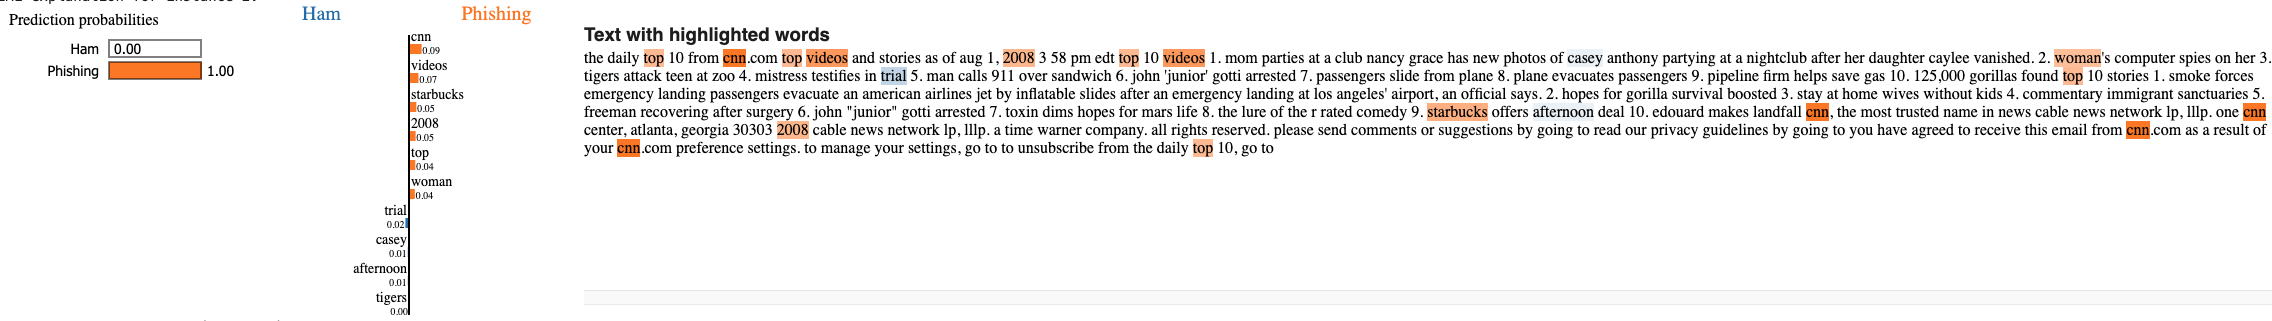
\includegraphics[scale=0.3,angle=90]{xai-visualisations/distilbert/Screenshot 2025-05-26 at 16.12.34.png}
    \caption{DistilBERT LIME explanation for Instance 1}
  \end{center}
\end{figure}

\newpage

\noindent Instance 2: Phishing email with urgent/action-oriented phrasing

\begin{itemize}
  \item \textbf{Original text snippet}: "\textit{approved, medicine fast delivery check out here}"
  \item \textbf{Model prediction}: Phishing (predicted class index: 1)
\end{itemize}

\noindent The final email instance was also classified as phishing, and the LIME explanation below demonstrates how terms such as "\textit{medicine}" (approx. weight \textbf{0.514}), "\textit{delivery}" (approx. weight \textbf{0.239})m and "\textit{fast}" (approx. weight \textbf{0.229}) all contribute strongly to the phishing classification. Terms like "\textit{approved}" did not have much of a significant impact. This shows the sensitive nature of the model to specific keywords.

\newpage

\vspace{0.5cm}
\begin{figure}[H]
  \begin{center}
    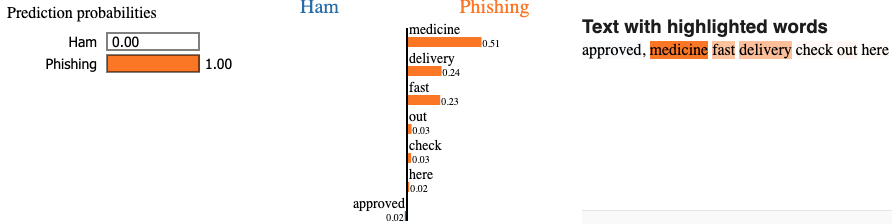
\includegraphics[scale=0.75,angle=90]{xai-visualisations/distilbert/Screenshot 2025-05-26 at 16.14.19.png}
    \caption{DistilBERT LIME explanation for Instance 2}
  \end{center}
\end{figure}
